\documentclass[12pt]{article}
\usepackage{graphicx}
\usepackage{amsmath}

\begin{document}
\begin{center}
\textbf\large{CHAPTER-7 \\ COORDINATE GEOMETRY}

\end{center}
\section*{Excercise 7.4}

\begin{enumerate}
\item Determine the ratio in which the line $2x+y \text{ } –\text{ } 4=0$ divides the line segment joining the points $\vec{A}(2, – 2) \text{ and } \vec{B}(3, 7)$.

\item Find a relation between $x$ and $y$ if the points $(x, y), (1, 2) \text{ and } (7, 0)$ are collinear.

\item Find the centre of a circle passing through the points $(6, – 6), (3, – 7) \text{ and } (3, 3)$.

\item The two opposite vertices of a square are $(–1, 2) \text{ and } (3, 2)$. Find the coordinates of the other two vertices.

\item The Class X students of a secondary school in Krishinagar have been allotted a rectangular plot of land for their gardening activity. Sapling of Gulmohar are planted on the boundary at a distance of 1m from each other. There is a triangular grassy lawn in the plot as shown in fig.\ref{fig:Fig1}. The students are to sow seeds of flowering plants on the remaining area of the plot.\\

\begin{figure}[!h]
	\begin{center} 
	    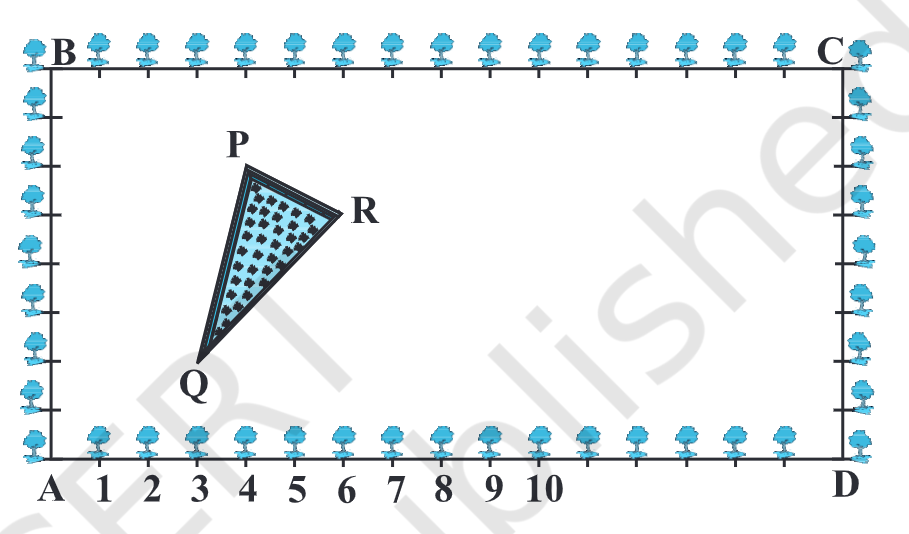
\includegraphics[width=\columnwidth]{figs/ss}
	\end{center}
\caption{}
\label{fig:Fig1}
\end{figure}

\begin{enumerate}
\item Taking A as origin, find the coordinates of the vertices of the triangle.\\
\item What will be the coordinates of the vertices of $\triangle$ PQR if C is the origin?\\
Also calculate the areas of the triangles in these cases. What do you observe?
\end{enumerate}


\item The vertices of a $\triangle$ABC are $\vec{A}(4,6), \vec{B}(1,5) \text{ and } \vec{C}(7,2)$. A line is drawn to intersect sides AB and AC at D and E respectively, such that $\frac{AD}{AB} = \frac{AE}{AC} = \frac{1}{4}$. Calculate the area of $\triangle$ADE and compare it with the area of the $\triangle$ABC.

\item Let $\vec{A}(4, 2), \vec{B}(6, 5) \text{ and } \vec{C}(1, 4)$ be the vertices of $\triangle$ABC.\\

\begin{enumerate}
\item The median from A meets BC at D. Find the coordinates of the point D.\\
\item Find the coordinates of the point P on AD such that $AP : PD = 2 : 1$\\
\item Find the coordinates of points Q and R on medians BE and CF respectively such that $BQ : QE = 2 : 1 \text{ and } CR : RF = 2 : 1$.\\
\item What do yo observe?\\
\textbf{Note} : The point which is common to all the three medians is called the centroid and this point divides each median in the ratio $2 : 1$.\\
If $A(x_{1},y_{1}), B(x_{2},y_{2}) \text{ and } C(x_{3},y_{3})$ are the vertices of $\triangle$ABC, find the coordinates of the centroid of the triangle.
\end{enumerate}


\item ABCD is a rectangle formed by the points $\vec{A}(–1, –1), \vec{B}(– 1, 4), \vec{C}(5, 4) \text{ and } \vec{D}(5, – 1)$. P, Q, R and S are the mid-points of AB, BC, CD and DA respectively. Is the quadrilateral PQRS a square? a rectangle? or a rhombus? Justify your answer.


\end{enumerate}



\end{document}
